
\chapter{Theory}%
\label{ch:theory}

\section{Anatomy}%
\label{sec:theory_anatomy}

The hand is a complex biomechanical system, comprised of many different bones, muscles, tendons, and ligaments. To explain different aspects of the hand in relation to one another, we use \textit{anatomical terminology} [\cite{AnatomicalTerminologySEER}], or more specifically \textit{anatomical directional terms}. Additionally when describing actions of muscles upon the skeleton, we use \textit{anatomical terms of movement} [\cite{TermsOfMovementTeachMeAnatomy}].

\subsection{Anatomical directional terms}%
\label{subsec:theory_anatomical_directional_terms}

Anatomical directional terms are used in relation to the \textit{anatomical position}, shown in Figure~\ref{fig:theory_anatomical_position}, where the body is assumed standing upright, with arms at the sides and palms facing forward. Relevant terms include: \textit{proximal}, \textit{distal}.

\begin{itemize}
    \item \textbf{Proximal} means toward or nearest the point of origin of a part.
    \item \textbf{Distal} means away from or farthest from the point of origin of a part.
\end{itemize}

\begin{figure}
    \centering
    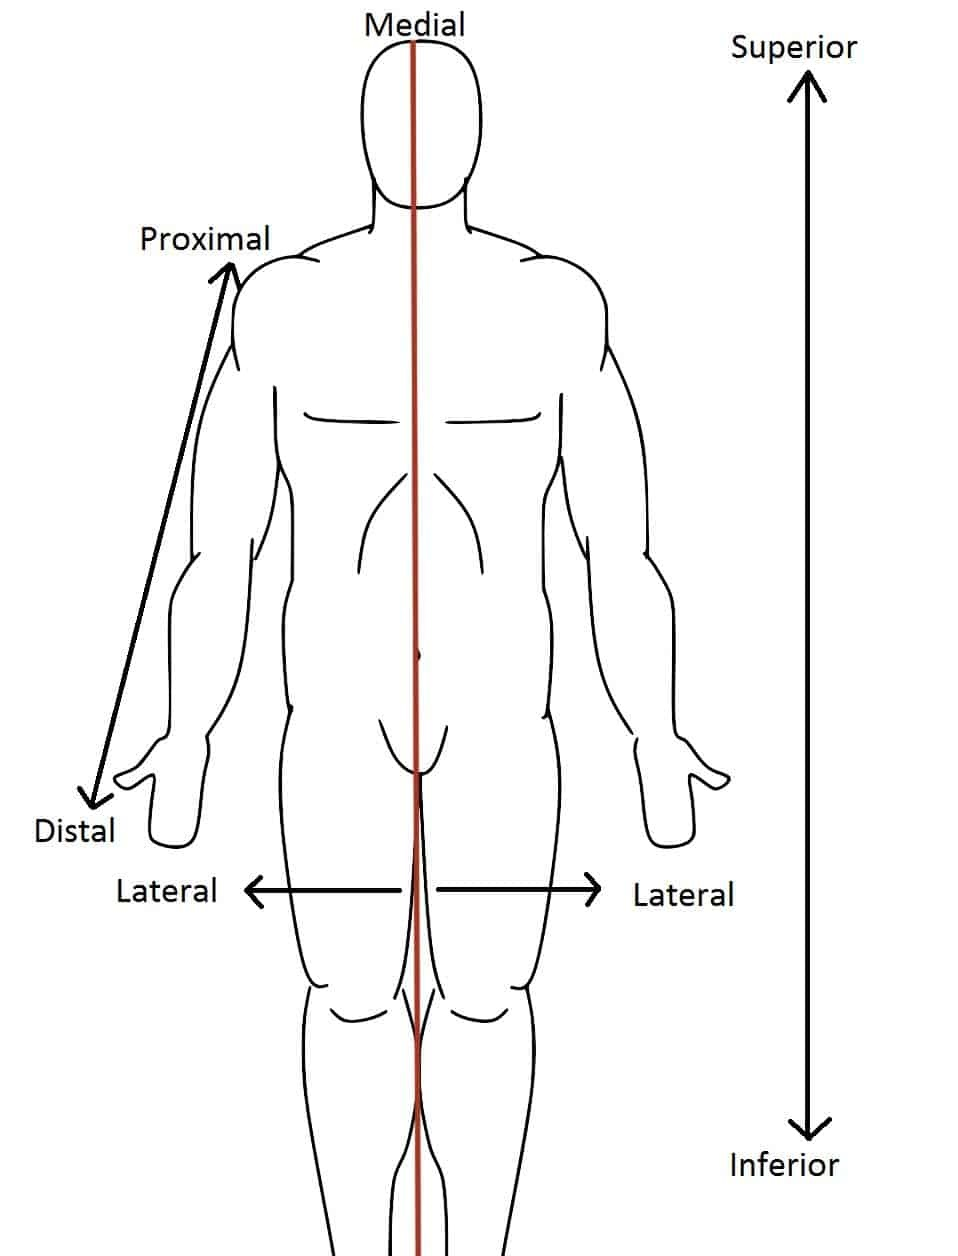
\includegraphics[width=0.5\textwidth]{Figures/Theory/anatomical_position.jpg}
    \caption{The anatomical position, with the corresponding directional terms. Image from~\cite{TeachMeAnatomyTermsOfLocation}.}%
    \label{fig:theory_anatomical_position}
\end{figure}

\subsection{Anatomical terms of movement}%
\label{subsec:theory_anatomical_terms_of_movement}
To explain the actions of muscles upon the skeleton, we use anatomical terms of movement, which describes the movement of a body part in relation to the anatomical position. Relevant terms include: \textit{flexion}, \textit{extension}, \textit{abduction}, \textit{adduction}.

\begin{itemize}
    \item \textbf{Flexion} is a movement that decreases the angle between two body parts.
    \item \textbf{Extension} is a movement that increases the angle between two body parts.
    \item \textbf{Abduction} is a movement away from the midline of the body.
    \item \textbf{Adduction} is a movement toward the midline of the body.
\end{itemize}

\begin{figure}[H]
    \centering
    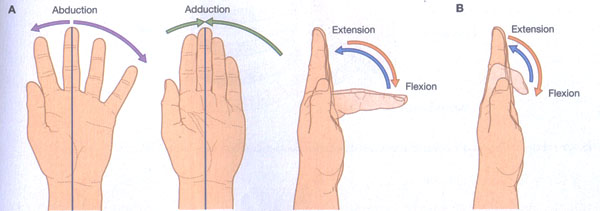
\includegraphics[width=0.8\textwidth]{Figures/Theory/anatomical_movements.jpg}
    \caption{Anatomical terms of movement. Image from~\cite{TermsOfMovementTeachMeAnatomy}.}%
    \label{fig:theory_anatomical_terms_of_movement}
\end{figure}

\subsection{Hand anatomy}%
\label{subsec:theory_hand_anatomy}
The hand is comprised of several bones, muscles, tendons, and ligaments. The bones, illustrated in Figure~\ref{fig:theory_hand_bones}, include the \textit{carpals}, \textit{metacarpals}, and \textit{phalanges}. The carpals make out the wrist, the metacarpals make out the palm, and the phalanges make out the fingers. The thumb has two phalanges, while the other fingers have three. The bones of interest are the phalanges (marked in green), as they are the ones being moved by the exoskeleton. The metacarpals are assumed stationary for the task at hand, as the exoskeleton will provide stiffness to the palm and wrist. 

The phalanges are further divided into three sections: the \textit{proximal phalanges}, the \textit{middle phalanges}, and the \textit{distal phalanges}. The proximal phalanges are the ones closest to the palm, while the distal phalanges are the ones furthest from the palm. The middle phalanges are the ones in between. The thumb does not have a middle phalanx, as it only has two phalanges.

\begin{figure}
    \centering
    \adjustbox{trim=0 {.30\height} 0 {.03\height}, clip, width=0.8\textwidth}{%
        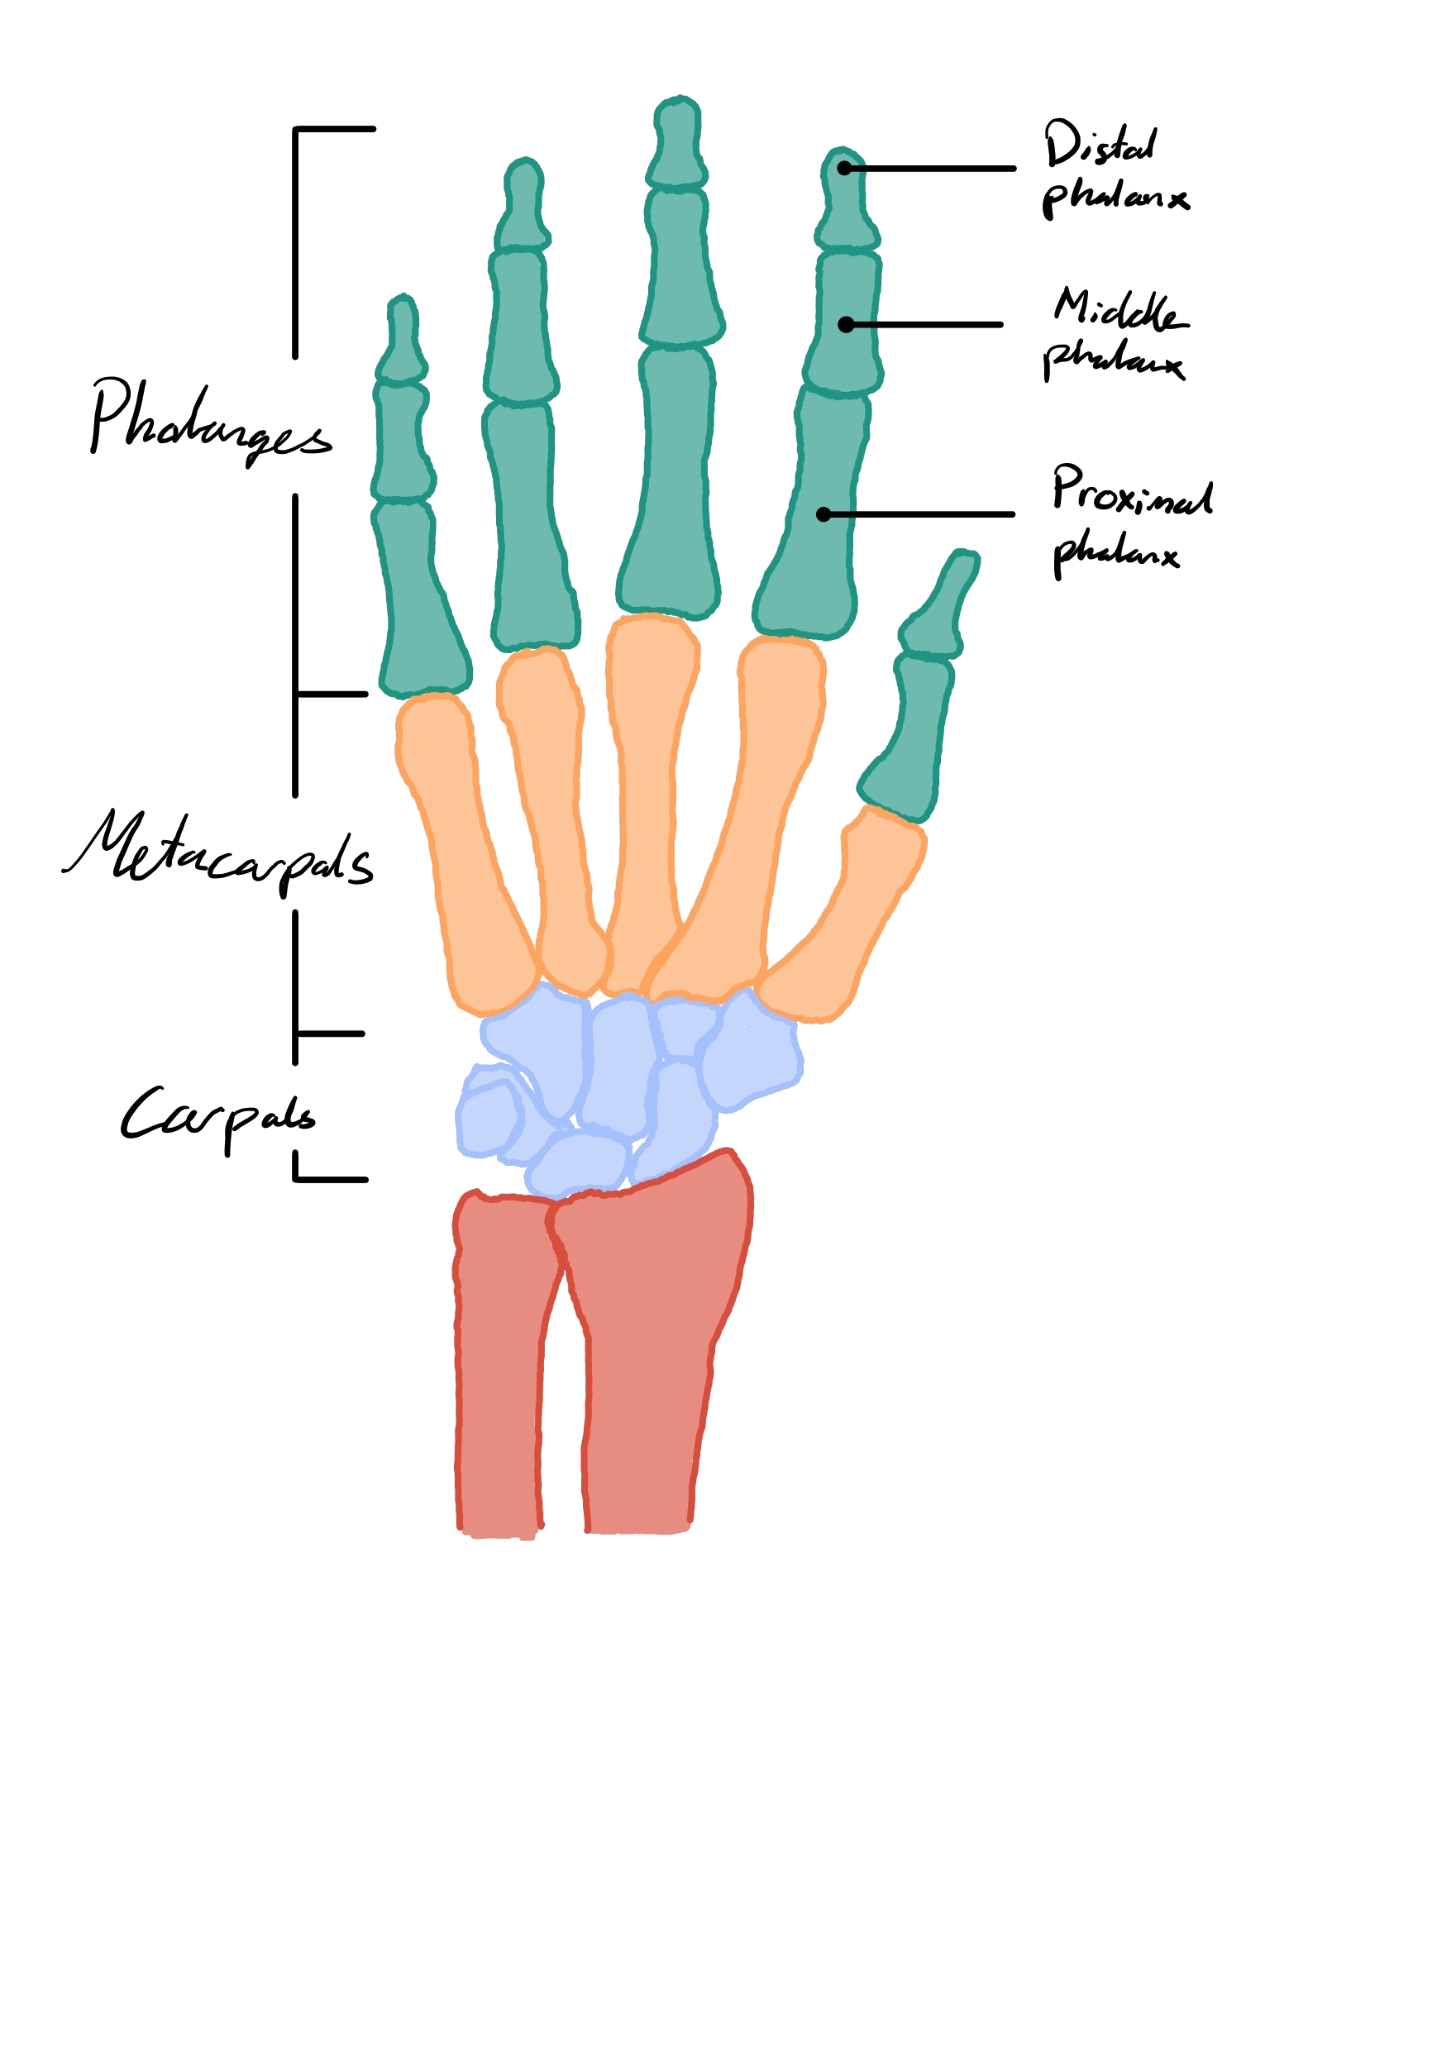
\includegraphics{Figures/Theory/hand_bones_no_bg.png}%
    }
    \caption{The bones of the hand. Image from author.}%
    \label{fig:theory_hand_bones}
\end{figure}

Further details about the joints are shown in Figure~\ref{fig:theory_hand_joints}. The joints of interest are the \textit{metacarpophalangeal joints} (MCP), the \textit{proximal interphalangeal joints} (PIP), and the \textit{distal interphalangeal joints} (DIP). The MCP joints are the ones between the metacarpals and the proximal phalanges, while the PIP joints are the ones between the proximal phalanges and the middle phalanges, and the DIP joints are the ones between the middle phalanges and the distal phalanges. The thumb only has an MCP joint and an interphalangeal joint (IP), as it does not have a middle phalanx.

At each of the joints, there are collateral ligaments that provide stability. For the PIP, IP and DIP joints, they provide stiffness that prevents side to side motion. For the MCP joints they're relaxed when the finger is extended, facilitating for adduction and abduction, but stiff when the finger is flexed.


\begin{figure}
    \centering
    \adjustbox{trim=0 {.30\height} 0 {.03\height}, clip, width=0.8\textwidth}{%
        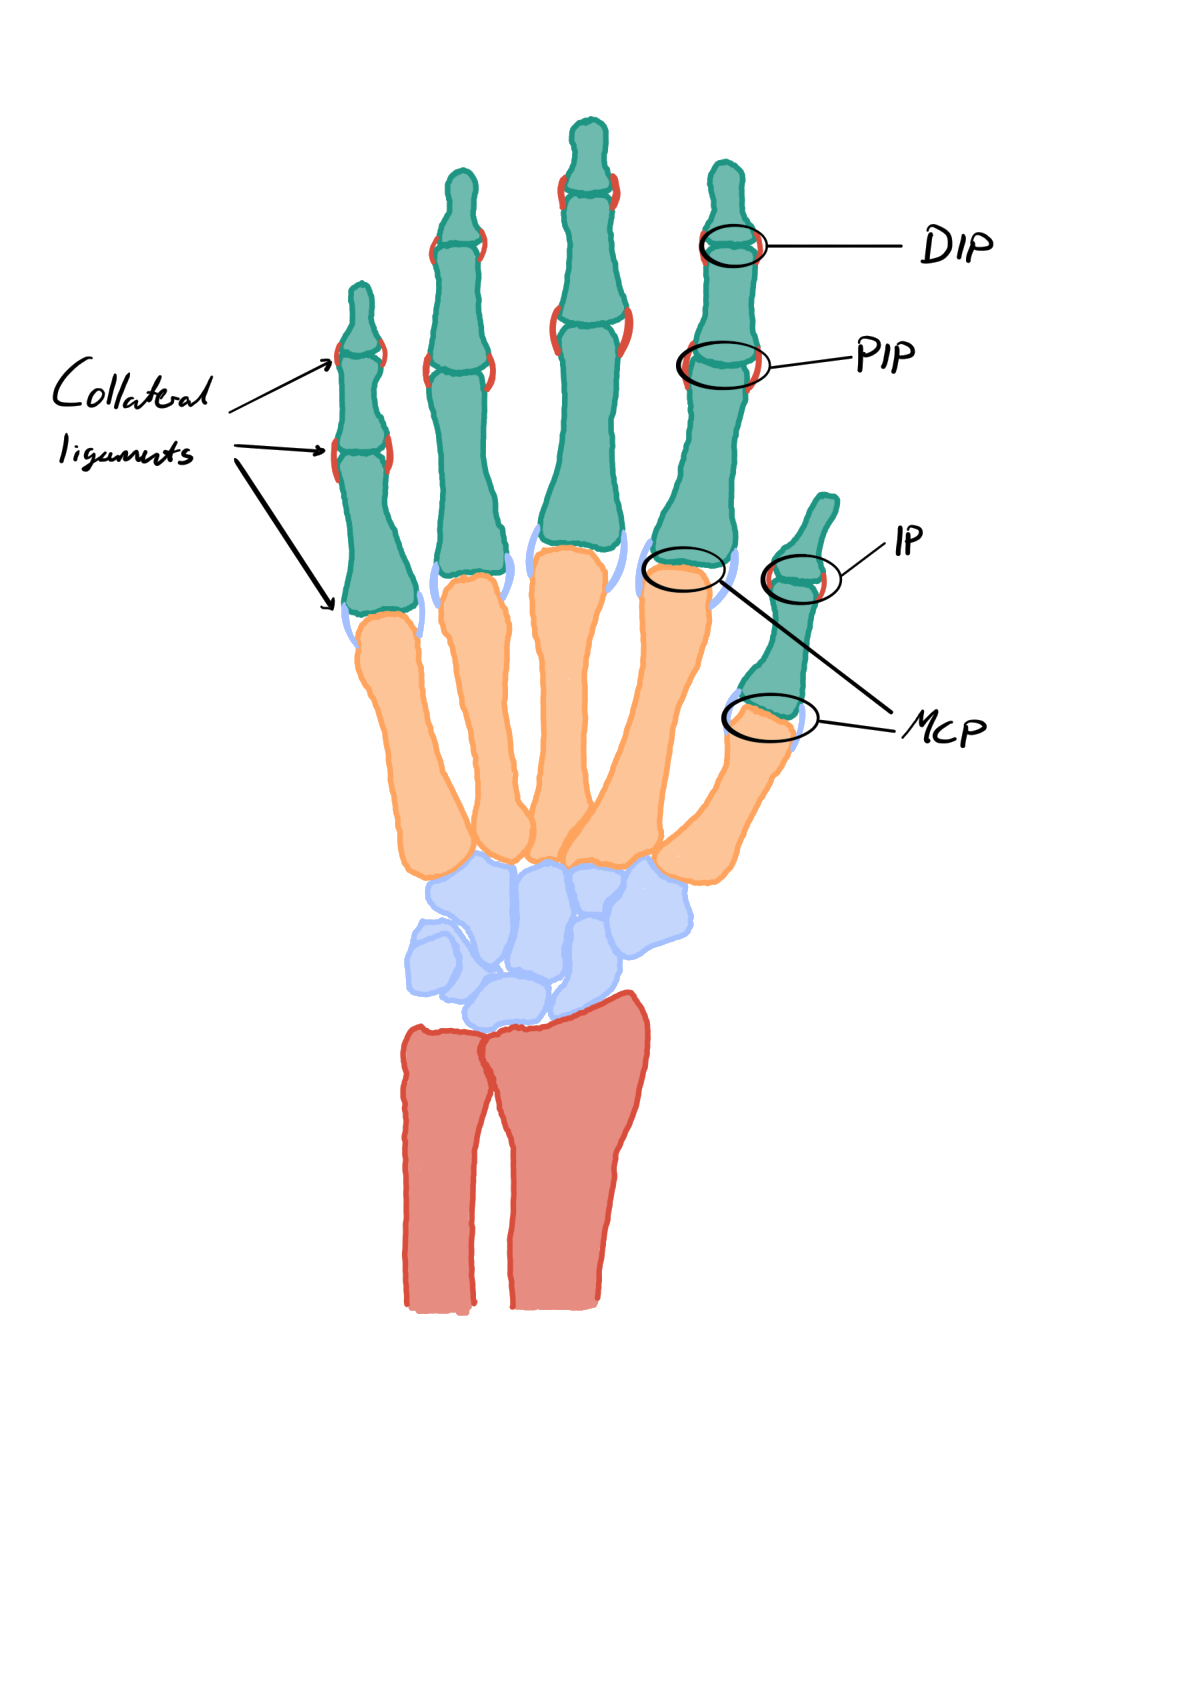
\includegraphics{Figures/Theory/hand_joints_2_pdf_no_bg.png}%
    }
    \caption{The joints of the hand. Image from author.}%
    \label{fig:theory_hand_joints}
\end{figure}

\section{Modelling}%
\label{sec:theory_modelling}

\subsection{Homogenous transformations}%
\label{subsec:theory_modelling_homogenous_transformations}

When modelling kinematic chains, we often need to move between frames. This often includes both rotation and translation. An efficient way to represent this is by using \textit{homogenous transformations}. 

\subsection*{Definition}
For a $2$D system, the rotation matrix for a counter-clockwise rotation by an angle $\theta$ is given by:

\begin{equation}
    \mathbf{R}(\theta) = \begin{bmatrix}
        \cos(\theta) & -\sin(\theta) \\
        \sin(\theta) & \cos(\theta)
    \end{bmatrix}.
\end{equation}

Given a translation vector from frame $i$ to frame $j$, written in terms of frame $i$, $\mathbf{d}_i^j = \begin{bmatrix}
    d_x^i \\
    d_y^i
\end{bmatrix}$, the homogenous transformation matrix from frame $j$ to frame $i$, describing the rotation $\theta$ and translation $\mathbf{d}_i^j$ from frame $i$ to frame $j$, can be expressed as:

\begin{equation}
    \label{eq:theory_homogenous_transformation}
    \mathbf{H}_j^i = \begin{bmatrix}
        \mathbf{R}(\theta) & \mathbf{d}_i^j \\
        \mathbf{0}_{1 \times 2} & 1
    \end{bmatrix}.
\end{equation}

Points represented in terms of homogenous transformations are represented as a 3D vector, where the first two elements represent the coordinates of the point in the plane, and the third element is always $1$. For example, a point $\mathbf{p}_n$ in frame $n$ with coordinates $(x,y)$ can be represented as:

\begin{equation}
    \mathbf{p}_n = \begin{bmatrix}
        p_x^n \\
        p_y^n \\
        1
    \end{bmatrix}.
\end{equation}

\subsection*{Useful properties}

Given a kinematic chain of size $n$, we can express the homogenous transformation from frame $n$ to frame $1$ as the product of the homogenous transformations between each consecutive frame:

\begin{equation}
    \label{eq:theory_homogenous_transformation_chain}
    \mathbf{H}_n^1 = \mathbf{H}_2^1 \mathbf{H}_3^2 \cdots \mathbf{H}_n^{n-1}.
\end{equation}

Given a point $\mathbf{p}_n$ in frame $n$, we can express it in frame $1$ as:

\begin{equation}
    \label{eq:theory_homogenous_transformation_chain_application}
    \mathbf{p}_1 = \begin{bmatrix}
        p_x^1 \\
        p_y^1 \\
        1
    \end{bmatrix} = \mathbf{H}_2^1 \mathbf{H}_3^2 \cdots \mathbf{H}_n^{n-1} \mathbf{p}_n = \mathbf{H}_n^1 \mathbf{p}_n.
\end{equation}

\section{Control}%
\label{sec:theory_control}

\subsection{State-Space representation}%
\label{subsec:theory_control_state_space}
A way to express a n'th order ordinary differential equation (ODE) is to express it as a system of n first order ODEs. This is called the \textit{state-space representation} of the system. A state-space representation commonly used in control theory for linear time-invariant (LTI) systems is the following:
\begin{equation}
\label{eq:theory_state_space_representation}
\begin{aligned}
    \dot{\mathbf{x}}(t) &= \mathbf{A}\mathbf{x}(t) + \mathbf{B}\mathbf{u}(t) + \mathbf{d}(t),\\
    \mathbf{y}(t) &= \mathbf{C}\mathbf{x}(t),
\end{aligned}
\qquad
\begin{aligned}
    \mathbf{x}(t) &\in \mathbb{R}^n, &
    \mathbf{u}(t) &\in \mathbb{R}^m, &
    \mathbf{y}(t) &\in \mathbb{R}^p, &
    \mathbf{d}(t) &\in \mathbb{R}^n, \\
    \mathbf{A}    &\in \mathbb{R}^{n \times n}, &
    \mathbf{B}    &\in \mathbb{R}^{n \times m}, &
    \mathbf{C}    &\in \mathbb{R}^{p \times n}. &&
\end{aligned}
\end{equation}

Here, $\mathbf{x}(t)$ is the state vector, which contains all the information about the system at time $t$. $\mathbf{u}(t)$ is the input vector at time $t$. $\mathbf{y}(t)$ is the output vector, which contains all the measurements of the system at time $t$. $\mathbf{d}(t)$ is a disturbance vector.

\subsection{Controllability}%
\label{subsec:theory_control_controllability}
A system is said to be \textit{controllable} if it is possible to drive the state of the system from any initial state to any desired final state in finite time, using an appropriate control input. For a LTI system, controllability can be determined by the rank of the controllability matrix $\mathcal{C}$, defined as:
\begin{equation}
    \mathcal{C} = [\mathbf{B}, \mathbf{A}\mathbf{B}, \mathbf{A}^2\mathbf{B}, \ldots, \mathbf{A}^{n-1}\mathbf{B}].
\end{equation}

If $\text{rank}(\mathcal{C}) = n$, where $n$ is the dimension of the state vector $\mathbf{x}$, then the system is controllable.

\subsection{MRAC}%
\label{subsec:theory_control_mrac}

\textit{Model Reference Adaptive Control} (MRAC) is a control strategy that aims to make the output of a system follow the output of a reference model, even in the presence of uncertainties or disturbances. The following definition of MRAC is based on \textcite[325--327]{ioannouRobustAdaptiveControl2012}. 

Given the nth order LTI-system in state-space form,

\begin{equation}
    \frac{\mathrm{d}}{\mathrm{d}t} \mathbf{x}(t) = \mathbf{A}\mathbf{x}(t) + \mathbf{B}\mathbf{u}(t), \quad \mathbf{x}(t) \in \mathbb{R}^n, \mathbf{u}(t) \in \mathbb{R}^m,
\end{equation}

and the reference model,

\begin{equation}
    \label{eq:theory_control_reference_model}
    \frac{\mathrm{d}}{\mathrm{d}t} \mathbf{x}_m(t) = \mathbf{A}_m\mathbf{x}_m(t) + \mathbf{B}_m\mathbf{r}(t), \quad \mathbf{x}_m(t) \in \mathbb{R}^n, \mathbf{r}(t) \in \mathbb{R}^m.
\end{equation}

The reference model and input $\mathrm{r}(t)$ are chosen so that $\mathbf{x}_m(t)$ represents the desired trajectory that $\mathbf{x}(t)$ should follow. Crucially, $\mathbf{A}_m$ must be a stable matrix, and $(\mathbf{A}, \mathbf{B})$ must be \textit{controllable} for this to work. If matrices $\mathbf{A}$ and $\mathbf{B}$ are known, then the control input $\mathbf{u}(t)$ can be designed as follows:

\begin{equation}
    \label{eq:theory_control_ideal_mrac_input}
    \mathbf{u}(t) = -\mathbf{K^*}\mathbf{x}(t) + \mathbf{L^*}\mathbf{r}(t),
    \quad \mathbf{K^*} \in \mathbb{R}^{m \times n}, \mathbf{L^*} \in \mathbb{R}^{m \times m}.
\end{equation}

This obtains the closed loop system:

\begin{equation}
    \frac{\mathrm{d}}{\mathrm{d}t} \mathbf{x}(t) = (\mathbf{A} - \mathbf{B}\mathbf{K^*})\mathbf{x}(t) + \mathbf{B}\mathbf{L^*}\mathbf{r}(t).
\end{equation}

If we choose $\mathbf{K^*}$ and $\mathbf{L^*}$ such that,

\begin{equation}
    \mathbf{A} - \mathbf{B}\mathbf{K^*} = \mathbf{A}_m, \quad \quad \mathbf{B}\mathbf{L^*} = \mathbf{B}_m,
\end{equation}

then the closed loop system becomes:

\begin{equation}
    \frac{\mathrm{d}}{\mathrm{d}t} \mathbf{x}(t) = \mathbf{A}_m\mathbf{x}(t) + \mathbf{B}_m\mathbf{r}(t).
\end{equation}

Hence the closed-loop dynamics of $\mathbf{x}(t)$ is the same to \cref{eq:theory_control_reference_model}, and $\mathbf{x}(t) \to \mathbf{x}_m(t)$ exponentially fast. But for most cases, $\mathbf{A}$ and $\mathbf{B}$ are not known, which means that $\mathbf{K^*}$ and $\mathbf{L^*}$ has to be estimated online. Assuming that $\mathbf{K^*}$ and $\mathbf{L^*}$ exist, we'll change the input in \cref{eq:theory_control_ideal_mrac_input} to:

\begin{equation}
    \label{eq:theory_control_mrac_input}
    \mathbf{u}(t) = -\mathbf{K}(t)\mathbf{x}(t) + \mathbf{L}(t)\mathbf{r}(t),
    \quad \mathbf{K}(t) \in \mathbb{R}^{m \times n}, \mathbf{L}(t) \in \mathbb{R}^{m \times m}.
\end{equation}

\subsubsection*{Adaptive Law}

Defining the tracking error $\mathbf{e}(t)$ as:

\begin{equation}
    \mathbf{e}(t) = \mathbf{x}(t) - \mathbf{x}_m(t).
\end{equation}

Solving for $\mathbf{P}$ for a $\mathbf{Q} =\mathbf{Q}^T > 0$ in the Lyapunov equation:

\begin{equation}
    \mathbf{A}_m^T\mathbf{P} + \mathbf{P}\mathbf{A}_m = -\mathbf{Q},
\end{equation}

we have the adaptive law:

\begin{equation}
    \begin{aligned}
        \dot{\mathbf{K}}(t) &= \mathbf{B}_m^T \mathbf{P} \mathbf{e} \mathbf{x}^T sgn(l), \\
        \dot{\mathbf{L}}(t) &= -\mathbf{B}_m^T \mathbf{P} \mathbf{e} \mathbf{r}^T sgn(l).
    \end{aligned}
\end{equation}

\cite{ioannouRobustAdaptiveControl2012} proves that with this adaptive law, that $\mathbf{K}(t)$, $\mathbf{L}(t)$, and $\mathbf{e}(t)$ are bounded, and the tracking error $\mathbf{e}(t) \to 0$ as $t \to \infty$.